\documentclass[a4paper,12pt]{article}
\usepackage{graphicx}
\usepackage[left=30mm, right=30mm, top=30mm, bottom=35mm]{geometry}
\usepackage{amsmath}
\usepackage{siunitx}
\usepackage{fancyhdr}
\usepackage{url}
\pagestyle{fancy}
%-------------------------------------------------------------------------------
\lhead{\textbf{Fall 2019}}
\rhead{\textbf{CE311K Intro to Computer Methods}}
\cfoot{\thepage}
%-------------------------------------------------------------------------------

\begin{document}
\begin{centering}
	\textbf{
		Assignment 03: Functions and modules\\
		Assigned: 22nd October 2019\\
		Due: 06th November 2019 at 5 PM\\
	}
\end{centering}


Note: Please upload your solution as an ipynb file to the Canvas page.

\vspace{1em}
 
 The purpose of this assignment is to develop your skills in writing functions and modules.
 
\begin{enumerate}
	
	\item Write a function to solve for the deflection of a beam supporting a uniformly distributed load $q$ to half its length as shown below. The beam could be both simply supported or fixed end. Assume by default the beam is simply supported, if not condition is specified. Write a Python function using conditional statements (if/else) to compute the deflection at any location $x$ along the length of the beam.

	\begin{figure}[ht]
		\centering
		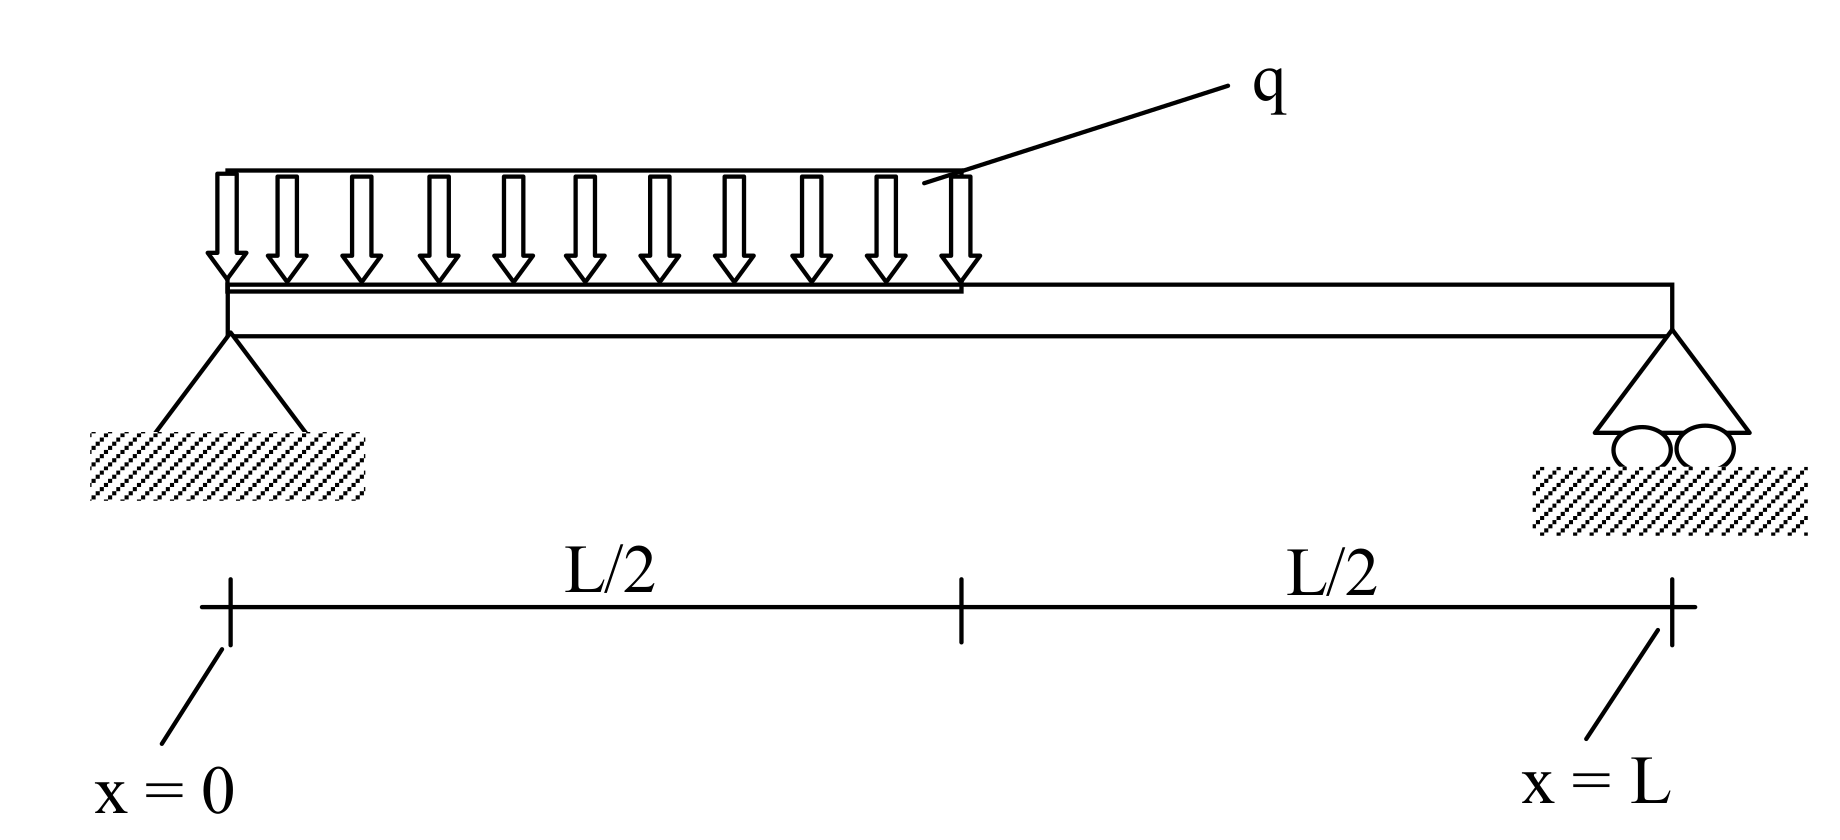
\includegraphics[width=0.6\textwidth]{ss-beam.png}
	\end{figure}

	For a given loading, the deflection of a simply supported beam $\delta(x)$ is:
	
	\begin{equation*}
		\delta(x) = \frac{q x}{384EI}(9L^3 - 24Lx^2 + 16x^3) \qquad 0 \le x \le \frac{L}{2}
	\end{equation*}
	
	and 

	\begin{equation*}
	\delta(x) = \frac{q L}{384EI}(8x^3 - 24Lx^2 + 17L^2x -L^3) \qquad \frac{L}{2} \le x \le L
	\end{equation*}
	
	For a given loading, the deflection of a fixed-end beam $\delta(x)$ is:
	
	\begin{equation*}
	\delta(x) = \frac{q x}{384EI}(11L^2x - 26Lx^2 + 16x^3) \qquad 0 \le x \le \frac{L}{2}
	\end{equation*}
	
	and 
	
	\begin{equation*}
	\delta(x) = \frac{q L}{384EI}( -L^3  + 8L^2x - 13Lx^2 + 6x^3) \qquad \frac{L}{2} \le x \le L
	\end{equation*}
	
	Note that $x < 0$ and $x > L$ are invalid locations. Use the following values for the various parameters involved in the above expressions:
	
	\begin{align*}
		q & = 4000 ~lb/ft\\
		L & = 20 ~ft\\
		EI & = 1.2x10^8 ~lb.ft^2
	\end{align*}
	
	Using these values, obtain the deflection at 3 locations: $x = L/4, L/2, 3L/4$ for both simply supported and fixed end beams.
	
	\item Create a user defined function called \verb|bisection| that implements the Bisection Method for computing the roots of equations. The equation that is to be solved should be defined in a separate user defined function called \verb|fn| and this function should be used within the bisection function. Use the bisection function within a Python script to find a root of an equation (see below).
	The arguments for the bisection function should be the initial guesses for $x0$ and $x1$.  The returned values from the bisection function should be the identified root, the number of iterations it took to obtain the root, and the error. 
	
	Your bisection function should stop iterating on the root when the approximate error ($\varepsilon_a$) is less than 0.01\%.

	Your program should contain extensive error checking. At a minimum, it must include the following features:
	\begin{enumerate}
		\item If the initial guesses are for an invalid range, then your program should return an error message.
		\item If the number of iterations it takes to converge to a solution exceeds 300, your program should produce an error message indicating that the solution could not be found within the specified number of iterations.
	\end{enumerate}

	When debugging your program it is important to solve a problem for which you know the answer. Use the simple polynomial for the accelerating car (given below):
	\begin{equation*}
	f(t) = 0.5 * a * t^2 + v_0 * t - d
	\end{equation*}
	Specify, $a = 0.6m/s^2$, $v_0 = 4.5 m/s$, and $d=50m$ and the approximate solution for the root is at $t\approx7.43s$.
	
	\item Develop a Python module called \verb|utmath| in the file  \verb|utmath.py| that computes the following.
	\begin{enumerate}
		\item \verb|utmath.pi|
		\item \verb|utmath.e|
		\item \verb|utmath.max(a, b)|
		\item \verb|utmath.min(a, b)|
		\item \verb|utmath.abs(x)|
		\item \verb|utmath.sin(x, tolerance)| (using an approximate solution for $\sin$ with a default argument of $1e-6$ of tolerance)
		\item \verb|utmath.cos(x, tolerance)| (using an approximate solution for $\cos$ with a default argument of $1e-3$ of tolerance)
	\end{enumerate}

	Using the defined modules compute the following:
	
	\begin{enumerate}
		\item \verb|utmath.pi * 5**2|
		\item \verb|print(utmath.e)|
		\item \verb|utmath.max(5, 3)|
		\item \verb|utmath.min(-3, -7)|
		\item \verb|utmath.abs(-5)|
		\item \verb|utmath.sin(0.5)|
		\item \verb|utmath.sin(0.5, 1e-8)|
		\item \verb|utmath.cos(1.5)|
		\item \verb|utmath.cos(1.5, 1e-6)|
	\end{enumerate}

\end{enumerate}

\end{document}

